Введение изменений в методику преподавания требует обосновании, выраженного в положительном изменении общественного блага.
Одним из подходов к его определению связан является функция суммарной пользы или счастья для всех членов общества.
Термин утилитарности и его экономически-философская трактовка описана в работах Иериямия Бентам \cite{bentham1996collected} в XVIII веке.
Популяризация и развития подхода связано с появлением теории игр в 20 веке \cite{nash1950bargaining} \cite{riley1981optimal} \cite{hurwicz1960optimality}.
В теории игр мотивы действий связывают с максимизацией скалярного потенциала называемого функцией утилитарности.
Полученные теорией игр результаты применяются при создании систем голосования \cite{gibbard1973manipulation},
проектировании транспортных систем \cite{harris1955fundamentals} и организации плана операций в сфере медицины \cite{roth2004kidney}.

\textit{Определение:} \textbf{Функция утилитарности} это концепция, разработанная в области экономики и используемая в теории принятия решений.
Она описывает способность индивида оценивать полезность или степень удовлетворения от различных вариантов действий или состояний.

Существует два принципиальных подхода к определению функцию утилитарности:\begin{itemize}
    \item в ординальном подходе утилитарное значение устанавливается относительно других альтернатив в порядке предпочтений; 
    \item в абсолютном --- утилитарное значение измеряется в конкретных единицах, что позволяет проводить количественные сравнения между 
    альтернативами и оценивать уровень удовлетворения количественно.
\end{itemize}

\textit{Определение:} \textbf{Равновесие по Нэшу} \cite{nash1950bargaining} --- состояние, в котором ни один игрок не может получить дополнительную выгоду от своих измененных действий, 
если другие игроки продолжат свои стратегии.
\begin{equation}
    \forall s_i \in S_i \rightarrow u_i(s_i^*,s^*_{-i}) \ge u_i(s_i,s_{-i}^*),
\end{equation}
где $u$ - функция утилиты, $S_i$ --- заданный набор игроков, $s_i^*$ - решение игрока $i$, соответсвующее равновесию по Нэшу,
$s_{-i} = S \backslash \{i\}$ --- обозначение исключения элемента множества $i$ из множества $S$.

Изучение равновесий по Нэшу в математических постановках позволяет задавать оптимальные системы правил, пресекающий
недобросовестный сговор. Классическим примером равновесия по Нэшу является дилемма заключенного, удобная к записи в виде
матрицы решений двух игроков (рис. \ref{dilem}). Модель определяет функцию полезности для совместных решений игроков.
При оптимальном задании правил наказания сообщника предпочтут не скрывать злодеяния сообщника.
\begin{equation}
    \forall s_i \in S_i u_i(s_i^*,s^*_{-i}),
\end{equation}

\begin{figure}[h]
    \centering
    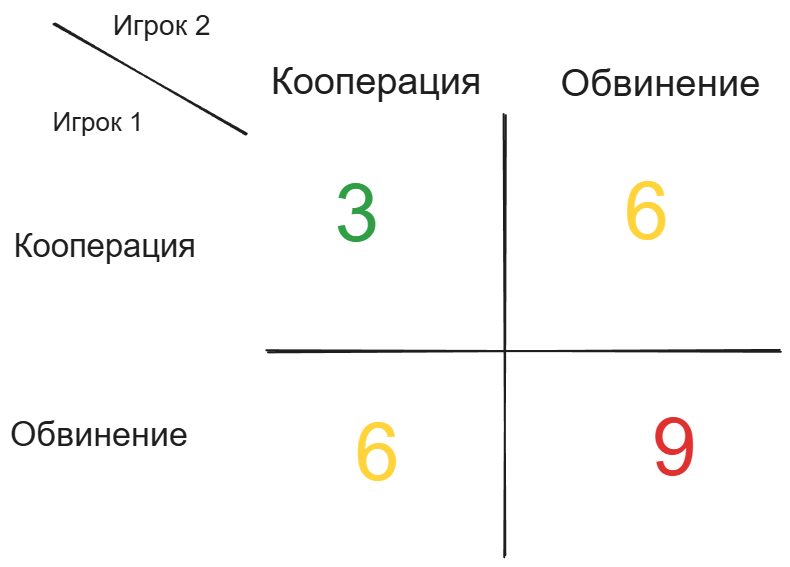
\includegraphics[width=0.6\textwidth]{assets/pedagogic/social/dilemma.excalidraw.png}
    \caption{Дилемма заключенного.}
    \label{dilem}
\end{figure}
